\begin{minipage}{0.55\textwidth}
\begin{align*}
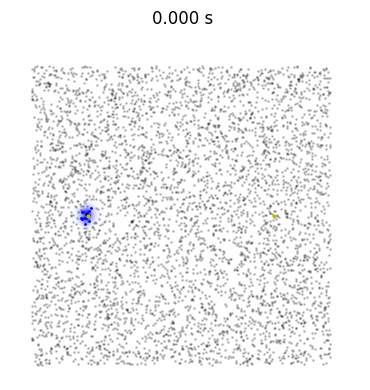
\includegraphics[width=0.49\textwidth]{simulation/8/frame_0.png}\hfill
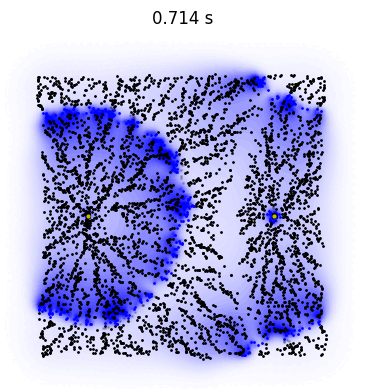
\includegraphics[width=0.49\textwidth]{simulation/8/frame_119.png}
\\[\smallskipamount]
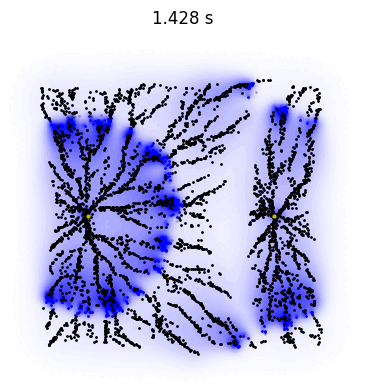
\includegraphics[width=0.49\textwidth]{simulation/8/frame_238.png}\hfill
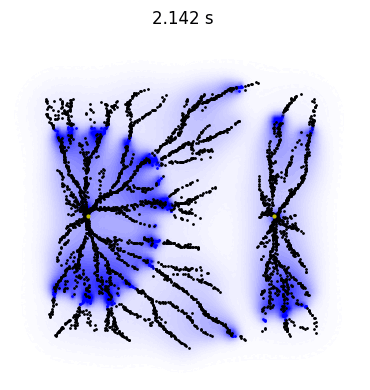
\includegraphics[width=0.49\textwidth]{simulation/8/frame_357.png}
\\[\smallskipamount]
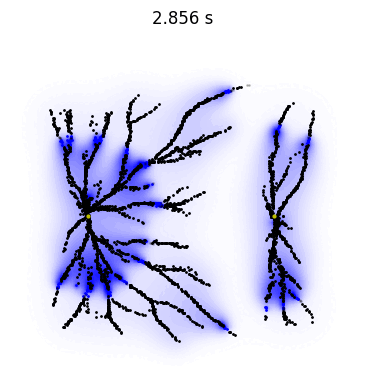
\includegraphics[width=0.49\textwidth]{simulation/8/frame_476.png}\hfill
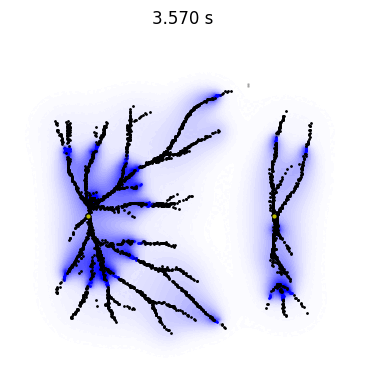
\includegraphics[width=0.49\textwidth]{simulation/8/frame_595.png}
\\[\smallskipamount]
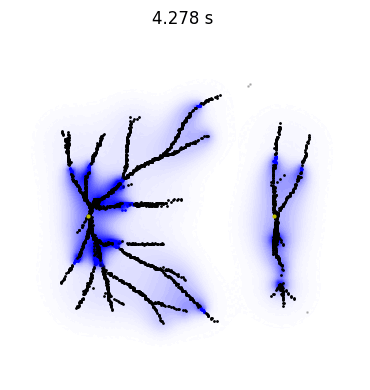
\includegraphics[width=0.49\textwidth]{simulation/8/frame_713.png}\hfill
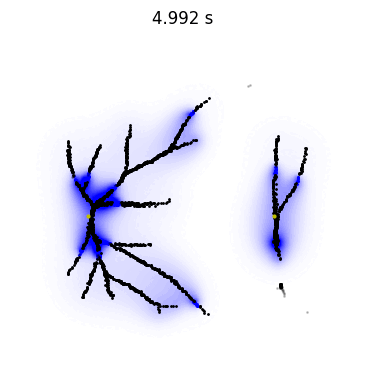
\includegraphics[width=0.49\textwidth]{simulation/8/frame_832.png}
\end{align*}
\end{minipage}
\begin{minipage}{0.45\textwidth}
\subsection{Out Of Sync Pacemakers}
Similar to the In Sync Pacemakers simulations we have a uniform distribution with two pacemakers.
This time we delayed the right pacemaker.
What one can observe is again very similar to the previous simulations.
At the place of the front collision a separation starts to form, however this time it is not a straight line but a hyperbola.
Also note that because the left pacemaker started early it had more time to \lq{}grab\rq{} particles and hence its structure is significantly bigger than the one to the right.
\end{minipage}